\chapter{Background and Theoritical Foundations}
\label{Chapter-Background}

% Todo: Edit to your liking
\section{Kubernetes}

\begin{figure}[h!]
  \centering
  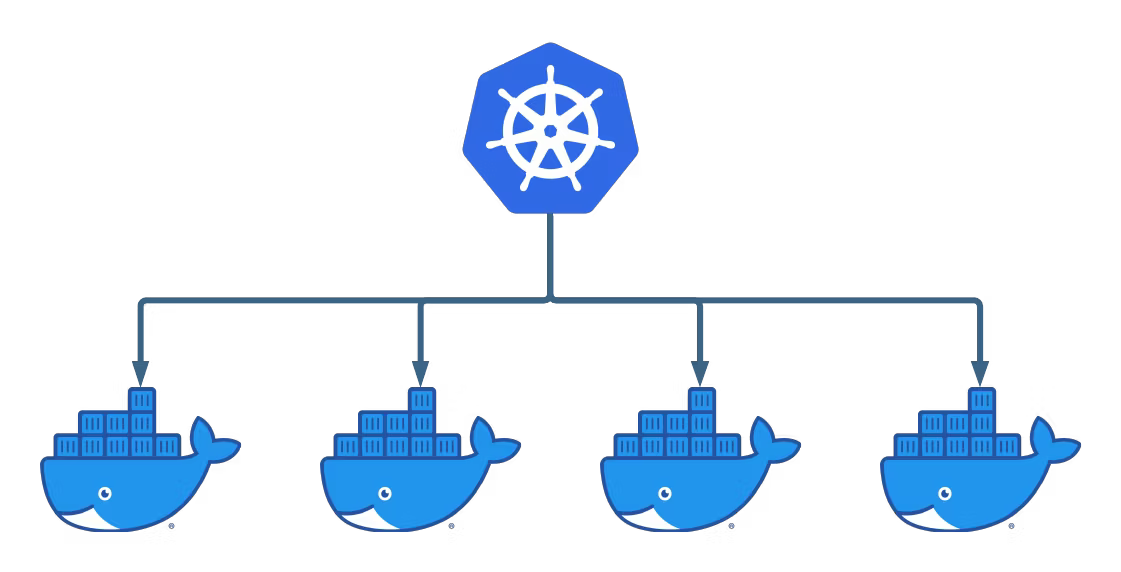
\includegraphics[width=1\textwidth]{Images/2024-04-10-k8s-vs-docker.png}
  \caption{Kubernetes}
  \label{fig:kubernetes}
\end{figure}

Kubernetes is an open-source container orchestration platform originally developed by Google~\cite{kubernetes-docs} 
and now maintained by the Cloud Native Computing Foundation (CNCF)~\cite{cncf-kubernetes}. It automates the deployment, 
scaling, and management of containerized applications across a cluster of machines. Kubernetes abstracts the infrastructure 
and provides primitives such as Pods, Deployments, Services, and Jobs, which allow developers to define complex systems 
declaratively.

% TODO more

In this project, Kubernetes serves as the core infrastructure layer for deploying isolated environments, managing job execution, 
and ensuring scalability and fault tolerance. The native support for namespaces, role-based access control (RBAC), and persistent 
volumes (PVs) makes it suitable for building multi-user platforms.
\section{Microservices}

The microservices architectural style structures an application as a collection of loosely coupled services, each responsible for 
a specific domain or capability~\cite{newman-microservices}. Microservices communicate primarily through lightweight mechanisms 
such as HTTP or messaging queues, and they are independently deployable.

This approach was adopted in the system to improve modularity and separation of concerns. For instance, authentication, job 
orchestration, and storage abstraction are implemented as separate services, allowing them to evolve independently and scale 
according to their individual loads.

\begin{figure}[h!]
  \centering
  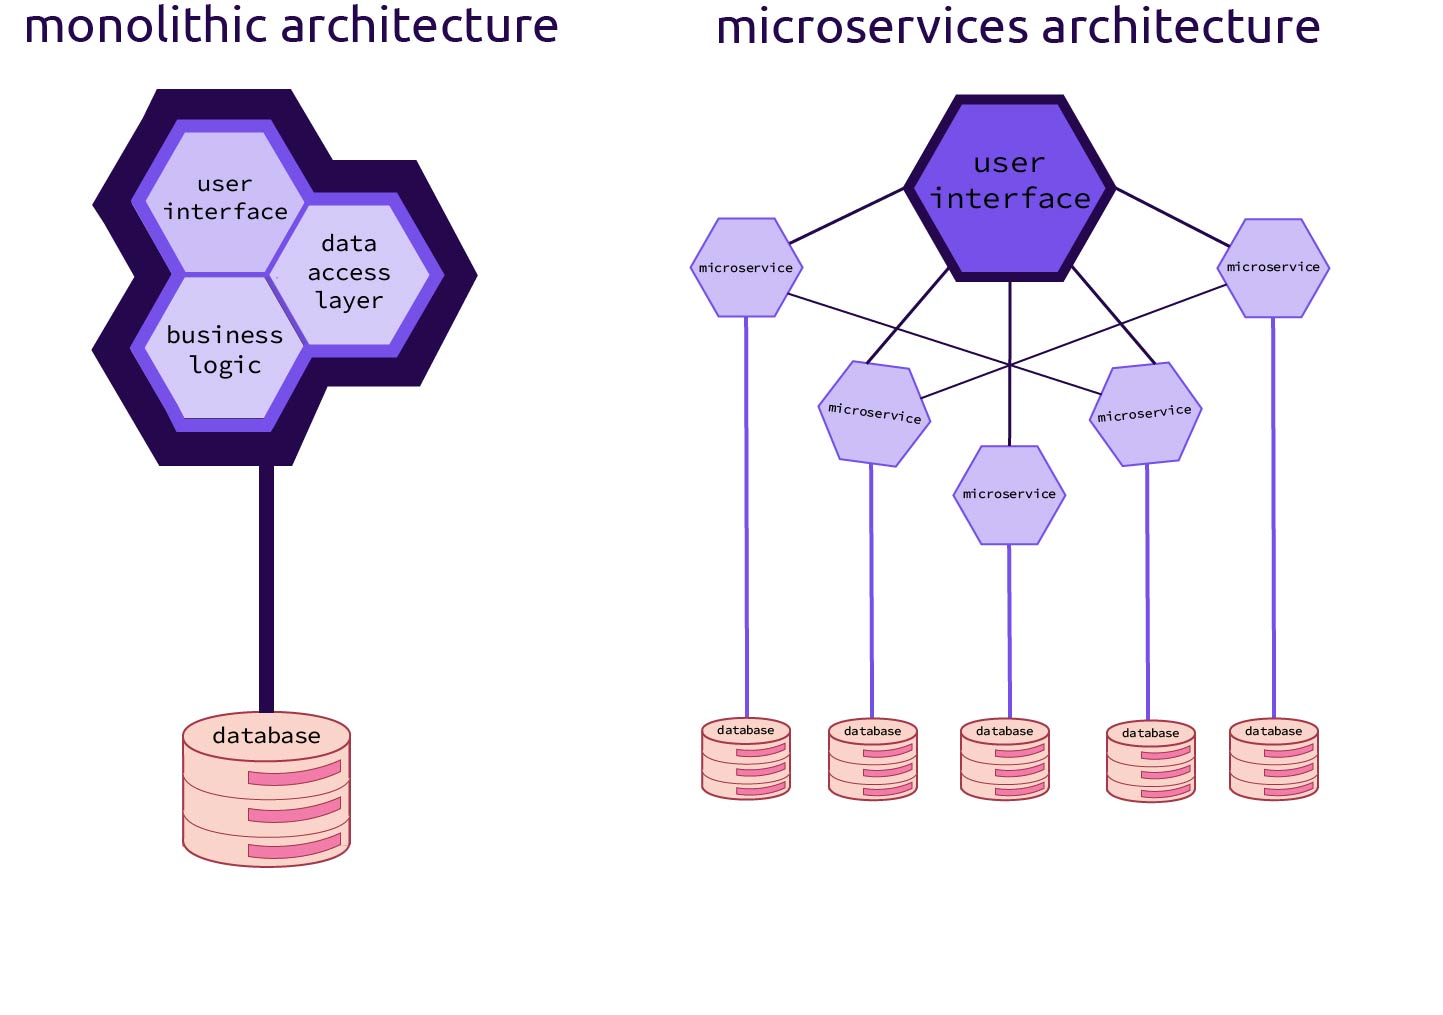
\includegraphics[width=1\textwidth]{Images/monoliths-vs-microservices-whats-the-difference_2.png}
  \caption{MicroServices vs Monolithic}
  \label{fig:microservicesVmonolithic}
\end{figure}

\section{Batch Job Execution}

Batch processing refers to the execution of non-interactive, background jobs that process data in large volumes~\cite{batch-processing}. 
Unlike real-time systems, batch jobs are scheduled and executed at specified times or on demand, often in isolated environments.

Kubernetes natively supports batch job execution through the \texttt{Job} and \texttt{CronJob} resources. In the designed system, 
batch jobs are launched on behalf of users to run data analysis scripts using containerized tools like DuckDB or Pandas, with each 
job being tracked and managed independently.

\section{MinIO}

\begin{figure}[h!]
  \centering
  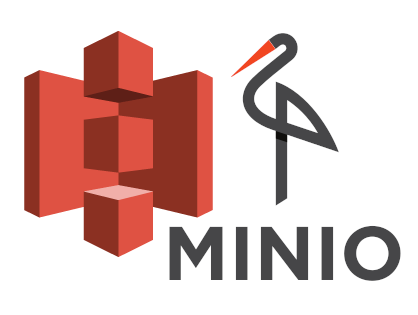
\includegraphics[width=0.5\textwidth]{Images/minIO.png}
  \caption{MinIO}
  \label{fig:minio}
\end{figure}

MinIO is a high-performance, Kubernetes-native object storage system compatible with the Amazon S3 API~\cite{minio-docs}. 
It is often used in cloud-native applications to store unstructured data such as logs, images, or datasets.

In the system, MinIO acts as the backend storage for user-uploaded files and job outputs. Its compatibility with S3 allows for flexible 
integration with analytics tools and easy management of large datasets without a traditional POSIX filesystem. 

Additionally, the imaged application tools used in the system are set with I/O on MinIO.
\section{DuckDB}

DuckDB is an in-process SQL OLAP (Online Analytical Processing) database management system optimized for analytical queries on 
columnar data~\cite{duckdb-paper}. Unlike traditional database servers, DuckDB runs directly within the host process and is designed for interactive 
analytics on local files such as CSV and Parquet. Its columnar storage model and vectorized query execution engine make it particularly 
suitable for analytical workloads involving large datasets.

DuckDB draws conceptual inspiration from systems like PostgreSQL and MonetDB, but emphasizes lightweight deployment and embeddability. 
It supports complex SQL queries, window functions, joins, and aggregations with high performance, while avoiding the operational 
complexity of client-server architectures.

\subsection*{Why DuckDB?}

\begin{figure}[h!]
  \centering
  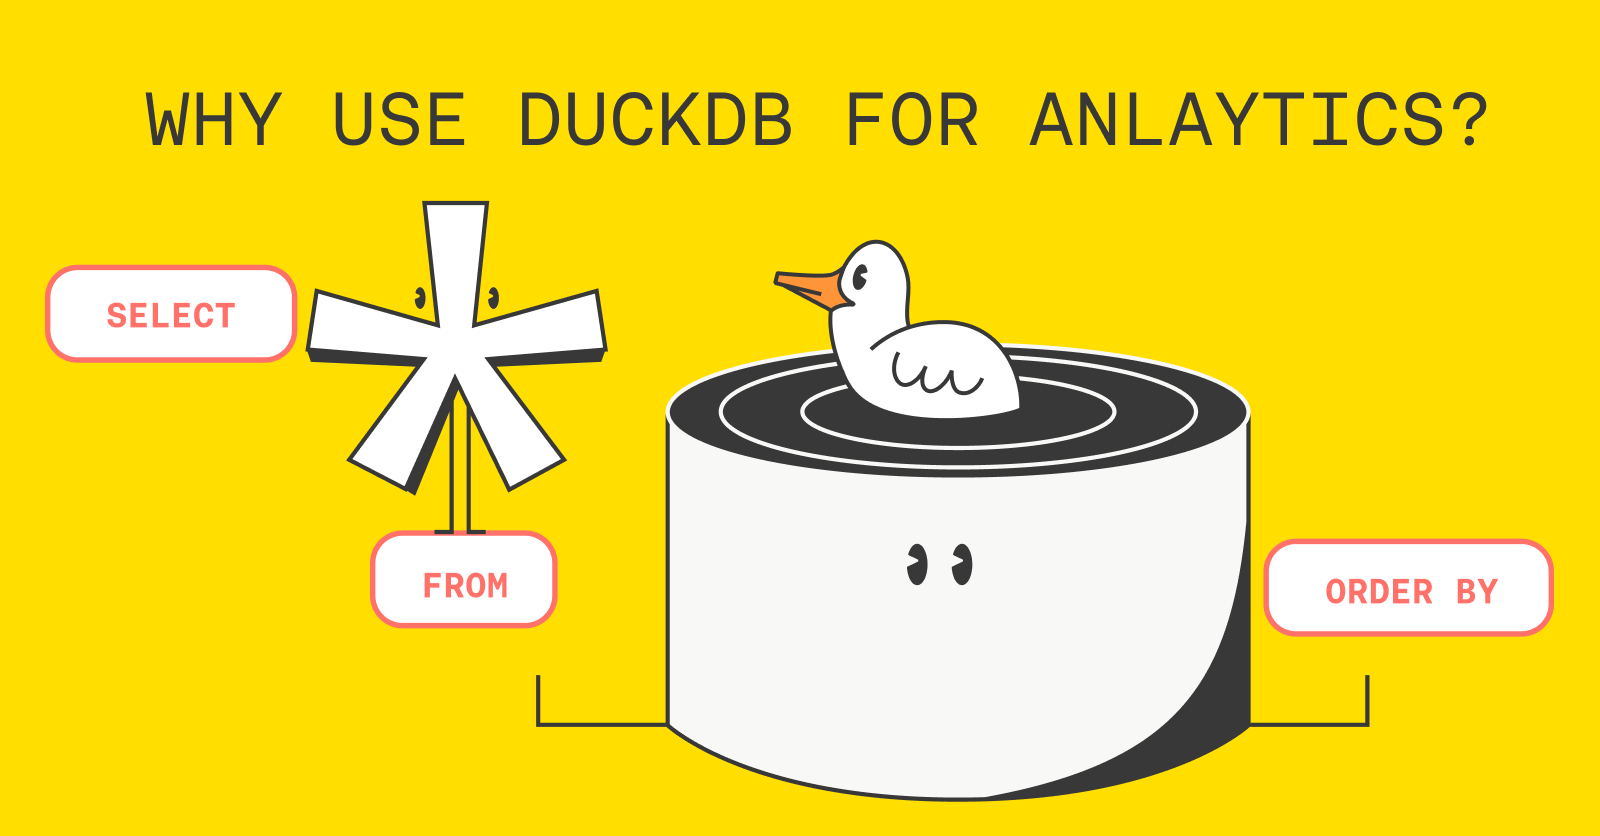
\includegraphics[width=1\textwidth]{Images/duckdb_for_analytics_1_c16a0acfc3.png}
  \caption{Why DuckDB}
  \label{fig:duckdb}
\end{figure}

DuckDB was chosen for this system due to several compelling advantages:

\begin{itemize}
    \item \textbf{Embeddability:} DuckDB can be run inside a container with no setup or external dependencies, making it ideal for 
    sandboxed job execution in Kubernetes.
    
    \item \textbf{Zero Configuration:} Users can query structured files (e.g., CSV, Parquet) without needing to first load data 
    into database tables, simplifying the user workflow.
    
    \item \textbf{Columnar Execution:} Optimized for analytical queries, DuckDB's columnar execution model enables efficient 
    processing of large datasets, particularly in filtering and aggregation operations.
    
    \item \textbf{File-Native Access:} Direct support for querying local data files stored on persistent volumes or object 
    storage simplifies integration with the storage layer (MinIO).
    
    \item \textbf{Lightweight and Fast:} Compared to heavier analytical engines, DuckDB has a small footprint and fast startup time, 
    which makes it suitable for short-lived Kubernetes jobs.
\end{itemize}

In this system, DuckDB is one of the containerized tools available for users to execute SQL-based data analysis jobs on uploaded datasets. 
Its integration enables users to perform complex transformations and analytics directly on their data without managing database 
infrastructure.

\section{SQLite}

\begin{figure}[h!]
  \centering
  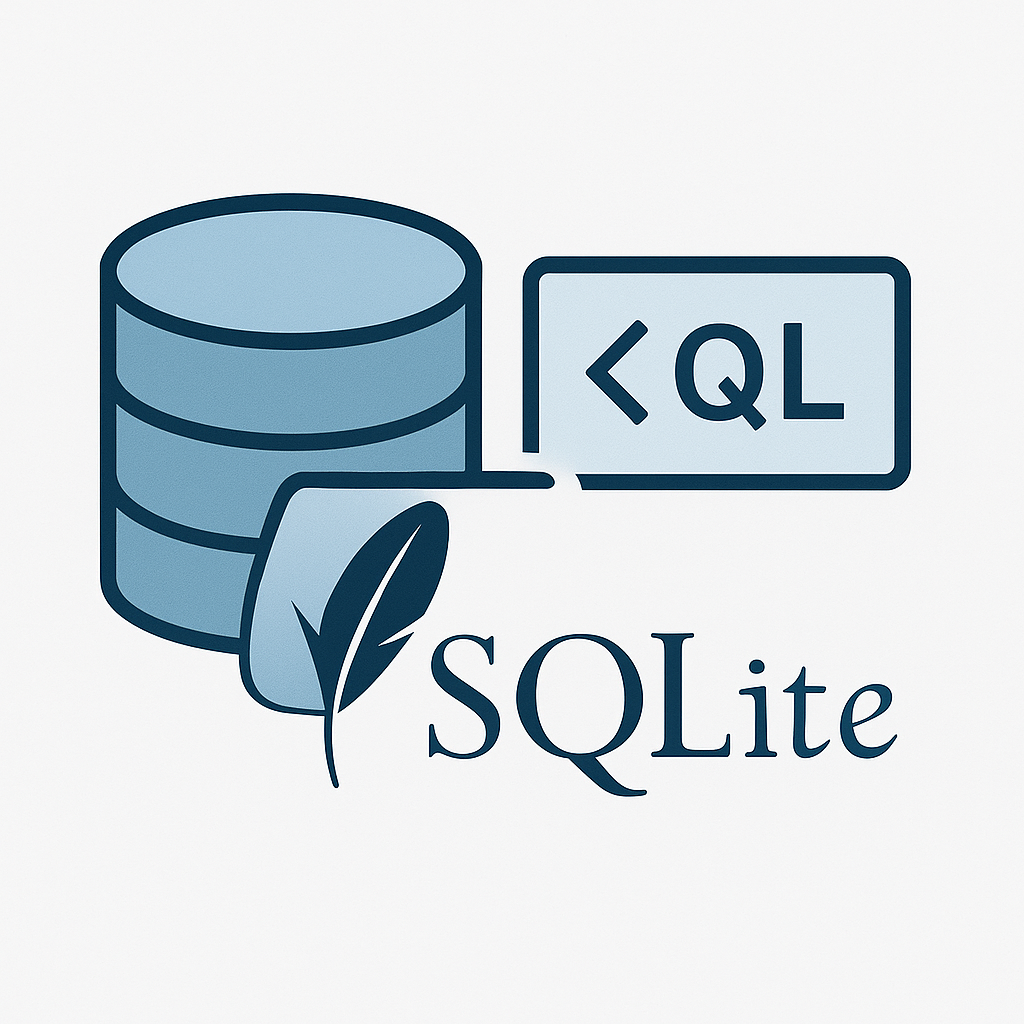
\includegraphics[width=0.5\textwidth]{Images/sqlite-chatgpt-img.png}
  \caption{SQLite}
  \label{fig:sqlite}
\end{figure}

SQLite is a lightweight, serverless, self-contained SQL database engine~\cite{sqlite-docs}. Unlike traditional client-server databases, 
SQLite operates directly on a single disk file and does not require a separate database server process. Its simplicity, low resource 
overhead, and zero-configuration nature make it an ideal choice for embedded applications and local data persistence.

In this system, SQLite is used as the backend storage mechanism for several services, including authentication (Minioth), 
filesystem metadata (Fslite), and job tracking (Uspace). Each service maintains its own isolated SQLite instance, ensuring 
modularity and local data consistency. The relational model of SQLite provides a robust framework for enforcing constraints, 
indexing, and transactional integrity, all while maintaining high performance for low- to moderate-volume workloads.

Due to its embeddable nature, SQLite enables rapid development and deployment of microservices without the overhead of managing 
a centralized database server. This aligns well with the platform’s goals of simplicity, portability, and lightweight infrastructure.


\section{WebSockets}
\begin{figure}[h!]
  \centering
  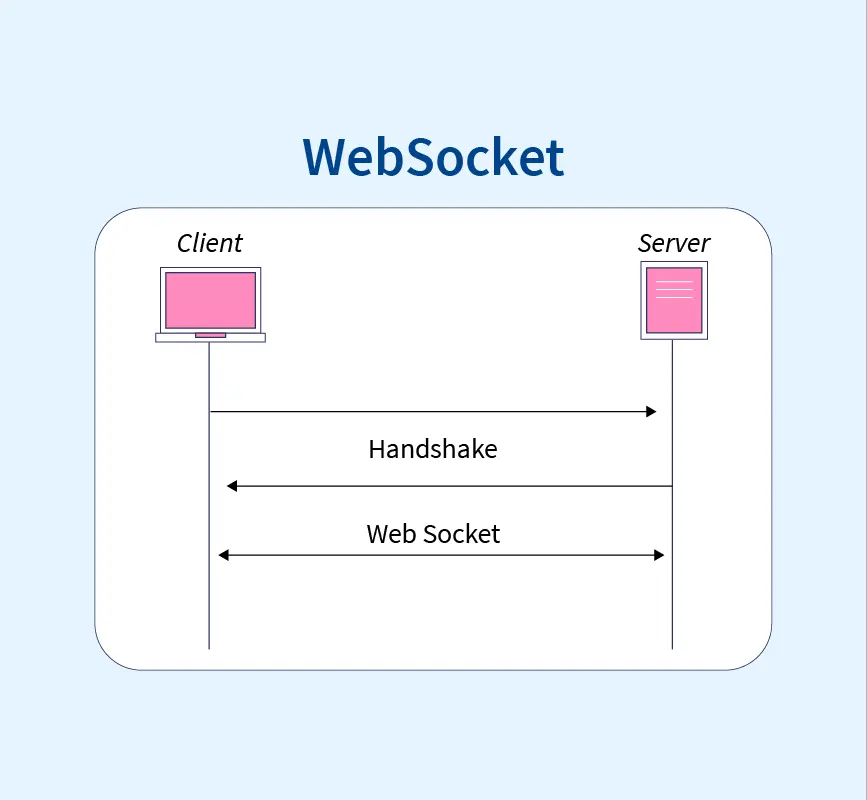
\includegraphics[width=0.8\textwidth]{Images/websockets-1.png}
  \caption{WebSockets}
  \label{fig:websockets}
\end{figure}

WebSockets provide a full-duplex communication channel over a single TCP connection, allowing real-time interaction between 
clients and servers~\cite{ietf-websocket}. Unlike traditional HTTP, WebSockets maintain a persistent connection, enabling low-latency communication.

The system utilizes WebSockets to allow users to interact with their environment in real time, including job monitoring and 
event-driven communication with backend services.
\section{Containers}

\begin{figure}[h!]
  \centering
  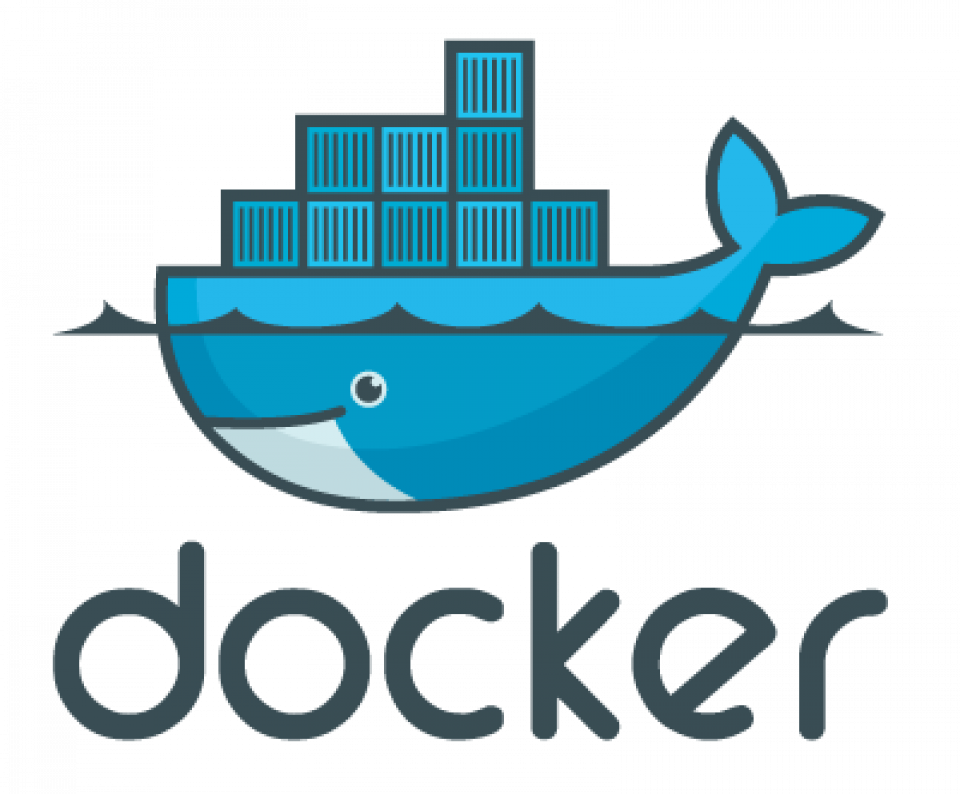
\includegraphics[width=0.5\textwidth]{Images/what-is-docker.png}
  \caption{Docker Containers}
  \label{fig:docker-containers}
\end{figure}

Containers are lightweight, portable units that package software with its dependencies and run isolated from the host 
system~\cite{docker-docs}. Technologies like Docker and container runtimes such as containerd have made containers a 
standard deployment model in modern systems.

In this system, each analytical job is executed within its own container, ensuring environment reproducibility and isolation 
between users. This also facilitates the inclusion of tools like Bash, Octave, and Python in a controlled, sandboxed manner.

The Microservices theirselves will be deployed as individual containers in collaboration with K8S.
\section{Multi-User System Design}

A multi-user system is one that supports concurrent access by multiple independent users, often with varying levels of access, 
permissions, and isolation. In such systems, key design considerations include authentication, authorization, resource sharing, 
and conflict avoidance~\cite{tanenbaum-os}.

The platform presented in this thesis implements a multi-user architecture where each user is assigned a secure, isolated environment. 
Users may upload datasets, execute jobs, and share resources depending on their group memberships and permissions. This design is 
inspired by UNIX-like models, incorporating user/group-based access control to enforce data protection and operational boundaries 
within a shared infrastructure.

\newpage
\section{Authentication Model}

Authentication is the process of verifying the identity of users before granting access to system resources~\cite{ferraiolo-auth}. 
In multi-user systems, secure and reliable authentication is foundational to ensuring that only authorized users can interact with 
sensitive data or operations.

The system utilizes a custom-built authentication service called \texttt{Minioth}, which follows a token-based authentication scheme 
using JSON Web Tokens (JWT). Upon successful login, users receive short-lived signed tokens that are used to authenticate future requests. 
This stateless approach enables efficient, scalable identity verification across distributed microservices, while also supporting user and 
group management for access control.

\newpage
\section{Cloud-Native Storage}

\begin{figure}[h!]
  \centering
  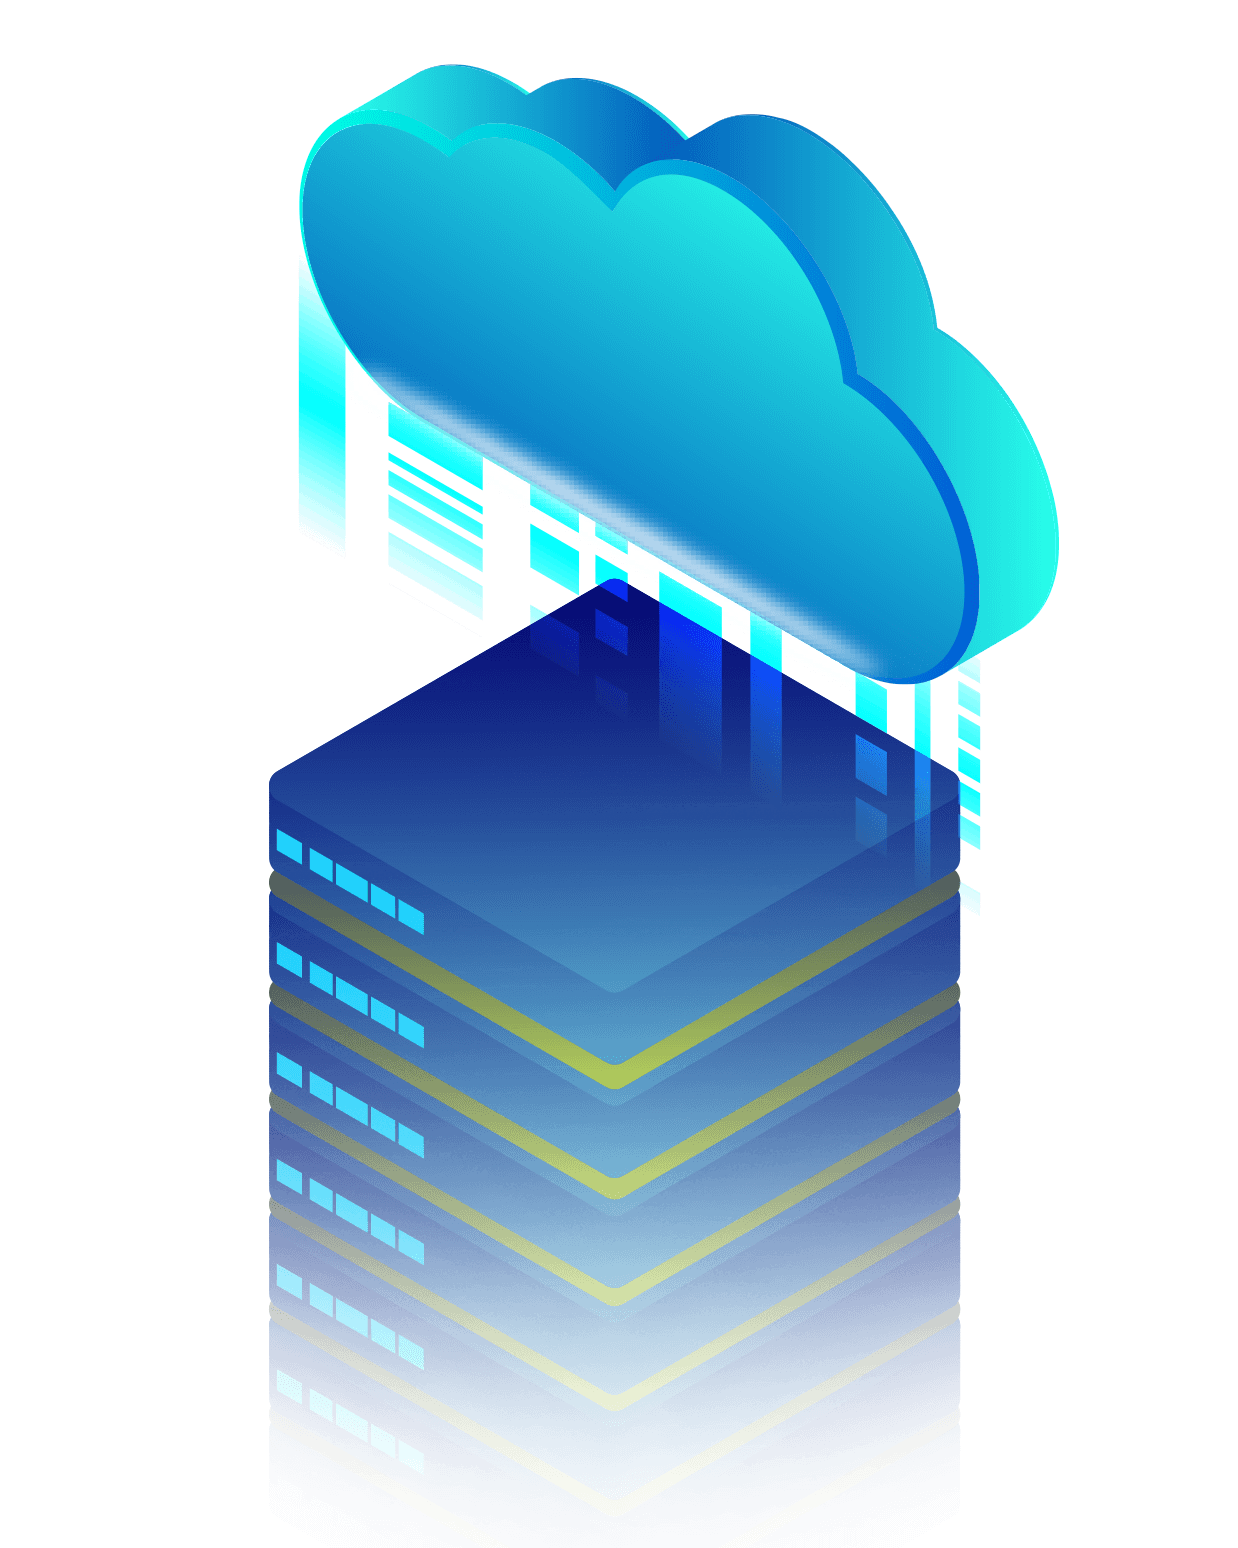
\includegraphics[width=0.4\textwidth]{Images/img-hybrid-cloud-engineer.png}
  \caption{CNS}
  \label{fig:cns}
\end{figure}

Cloud-native storage refers to storage systems designed to operate within cloud environments, typically containerized and orchestrated 
via platforms like Kubernetes~\cite{cncf-storage}. Unlike traditional block or file-based storage, cloud-native storage solutions are 
optimized for dynamic workloads, scalability, and high availability.

In this system, MinIO—a cloud-native object storage service compatible with Amazon S3—is used to store user data and job outputs. 
Object storage offers flexibility in managing large, unstructured datasets, and integrates seamlessly with Kubernetes via 
Persistent Volume Claims (PVCs). Cloud-native storage allows the system to dynamically provision isolated storage volumes for each 
user or job, supporting scalable and fault-tolerant operations.

